\documentclass[12pt,spanish,openany,letterpaper,pagesize]{scrbook}
\usepackage[utf8]{inputenc}
\usepackage[spanish]{babel}%escribir con acentos sin necesidad de comandos \'{} .
\usepackage{fancyhdr}
%\usepackage{epsfig}
\usepackage{epic}
\usepackage{eepic}
\usepackage{amsmath, amssymb, amsthm, latexsym, graphics, graphpap, layout, wasysym, multicol, enumerate,amsfonts,mathrsfs}
\usepackage{graphics,lscape}
\usepackage[mathscr]{euscript}
\usepackage{xcolor}
\usepackage{verbatim}
\usepackage{booktabs}
\usepackage{float}
\usepackage{hyperref}
\usepackage{threeparttable}
\usepackage{amscd}
\usepackage{here}
\usepackage[pdftex]{graphicx}
\usepackage{lscape}
\usepackage{tabularx}
\usepackage{subfigure}
\usepackage{longtable}
\usepackage{geometry}
\usepackage{cite}
\usepackage{algorithmic}
\usepackage{diagbox}
\usepackage{array,multirow}
\usepackage[all]{ xy}

\usepackage{rotating} %Para rotar texto, objetos y tablas seite. No se ve en DVI solo en PS. Seite 328 Hundebuch
                        %se usa junto con \rotate, \sidewidestable ....
                        

\renewcommand{\theequation}{\thechapter-\arabic{equation}}
\renewcommand{\thefigure}{\textbf{\thechapter-\arabic{figure}}}
\renewcommand{\thetable}{\textbf{\thechapter-\arabic{table}}}

\pagestyle{fancyplain}%\addtolength{\headwidth}{\marginparwidth}
\textheight22.5cm \topmargin0cm \textwidth16.5cm
\oddsidemargin0.5cm \evensidemargin-0.5cm%
\renewcommand{\chaptermark}[1]{\markboth{\thechapter\; #1}{}}
\renewcommand{\sectionmark}[1]{\markright{\thesection\; #1}}
\lhead[\fancyplain{}{\thepage}]{\fancyplain{}{\rightmark}}
\rhead[\fancyplain{}{\leftmark}]{\fancyplain{}{\thepage}}
\fancyfoot{}
\thispagestyle{fancy}%

\addtolength{\headwidth}{0cm}
\unitlength1mm %Define la unidad LE para Figuras
%\mathindent0cm %Define la distancia de las formulas al texto,  fleqn las %descentra
\marginparwidth0cm
\parindent0cm %Define la distancia de la primera linea de un parrafo a la margen

%Para tablas,  redefine el backslash en tablas donde se define la posici\'{o}n del texto en las
%casillas (con \centering \raggedright o \raggedleft)
\newcommand{\PreserveBackslash}[1]{\let\temp=\\#1\let\\=\temp}
\let\PBS=\PreserveBackslash

%Espacio entre lineas
\renewcommand{\baselinestretch}{1.1}

%Neuer Befehl f\"{u}r die Tabelle Eigenschaften der Aktivkohlen
\newcommand{\arr}[1]{\raisebox{1.5ex}[0cm][0cm]{#1}}

%Neue Kommandos
\usepackage{Befehle}
%Inicio del documento. Tener en cuenta que hay archivos auxiliares

\newtheorem{teor}{Teorema}[section]
\theoremstyle{definition}
\newtheorem{definition}[teor]{Definición}
\theoremstyle{example}
\newtheorem{example}[teor]{Ejemplo}
\newtheorem{lema}[teor]{Lema}
\newtheorem{afirmacion}[teor]{Afirmación}
\newtheorem{proposicion}[teor]{Proposición}
\newtheorem{coro}[teor]{Corolario}
\newtheorem{ole}[teor]{Conjetura}
%\theoremstyle{proposicion}

%\def\proof{\paragraph{Demostración:\\}}%\begin{proof}
%\def\endproof{\hfill$\blacksquare$}%\end{proof}

\begin{document}
\pagenumbering{roman}
%\newpage
%\setcounter{page}{1}
\begin{center}
\begin{figure}
\centering%

\includegraphics[scale=0.4]{Imagenes/logo_1.png}
%{file=uc.jpg,scale=1}%
\end{figure}
\thispagestyle{empty} \vspace*{2.0cm} \textbf{\huge
Predicción del comportamiento de una enfermedad simulada en autómatas celulares con un algoritmo propuesto en redes neuronales}\\[6.0cm]
\Large\textbf{Jorge Andrés Ibáñez Huertas}\\[4.0cm]
\small Universidad Central\\
Departamento de Matemáticas\\
Bogotá, Colombia\\
2021\\
\end{center}

\newpage{\pagestyle{empty}\cleardoublepage}

\newpage
\begin{center}
\thispagestyle{empty} \vspace*{0cm} \textbf{\huge
Predicción del comportamiento de una enfermedad simulada en autómatas celulares con un algoritmo propuesto en redes neuronales}\\[3.5cm]
\Large\textbf{Jorge Andrés Ibáñez Huertas}\\[3.0cm]
\small Trabajo de grado presentado como requisito parcial para optar al
t\'{\i}tulo de:\\
\textbf{Matemático}\\[3.0cm]
Director:\\
Carlos Isaac Zainea\\[3.5cm]
Universidad Central\\
Departamento de Matemáticas\\
Bogotá, Colombia\\
2021\\
\end{center}

\newpage{\pagestyle{empty}\cleardoublepage}

% \newpage
% \thispagestyle{empty} \textbf{}\normalsize
% \\\\\\%
% \textit{"Tan sólo por la educación puede el hombre llegar a ser hombre.\\ El hombre no es más que lo que la educación hace de él"\\
% \textit{Immanuel Kant}}\\[4.0cm]

\begin{flushright}
\begin{minipage}{8cm}
    \noindent
        \small
\end{minipage}
\end{flushright}

\newpage{\pagestyle{empty}\cleardoublepage}

\newpage
\thispagestyle{empty} \textbf{}\normalsize
\\\\\\%
\textbf{\LARGE Agradecimientos}\\

% Agradezco a mis padres Roosvelt Rivera y Angelica Useche por los años de apoyo incondicional en mis años de estudio, además de la profesora Edel María Serrano Iglesias (Q.E.P.D) sin la cuál no hubiera entrado al mundo de las matemáticas.\\
% También agradezco a los profesores que a lo largo de la carrera estuvieron dispuestos a enseñar y guiar con incontable paciencia y dedicación, entre ellos: Xiomara Rojas, Diana Herrera, Diana Pulido, Isaac Zainea, Miguel Pachón, Henry Naranjo, Fabián Sánchez, Nicolás Avilán y mi director de tesis Henry Sánchez.

\newpage{\pagestyle{empty}\cleardoublepage}

\newpage
\textbf{\LARGE Resumen}\\

% En este trabajo se desarrollan los resultados obtenidos en el artículo  de Morales \& Arbieto,  específicamente la distancia $GH^0$ dada en ese manuscrito. Una vez se haya comprendido la fundamentación y  analizado algunas propiedades de dicha métrica, se procederá a estudiar la estabilidad topológica de las dinámicas sobre espacios compactos utilizando en principio la noción de Walters con una métrica $C^0$. Luego, se define y analiza la noción de $GH$-estabilidad  resaltando la relación que existe entre ambas nociones.\\

\textbf{\LARGE Abstract}\\\\

% In this work the results obtained in the article by Morales \& Arbieto are developed, specifically, the distance $ GH^0$ given in the article. Once the foundation is understood and some properties of that metric have been analyzed, we will proceed to study the topological stability of the dynamics on compact spaces using a notion given by Walters with a  $C^0$-metric. After that, will be defined and analyzed the $GH$-stability notion highlighting the relationship between both notions.

\renewcommand{\tablename}{\textbf{Tabla}}
\renewcommand{\figurename}{\textbf{Figura}}
\renewcommand{\listtablename}{Lista de Tablas}
\renewcommand{\listfigurename}{Lista de Figuras}
\renewcommand{\contentsname}{Contenido}

%\newcommand{\clearemptydoublepage}{\newpage{\pagestyle{empty}\cleardoublepage}}
\cleardoublepage
\addcontentsline{toc}{chapter}{Lista de figuras} % para que aparezca en el indice de contenidos
\listoffigures % indice de figuras

%\cleardoublepage
%\addcontentsline{toc}{chapter}{Lista de tablas} % para que aparezca en el indice de contenidos

\tableofcontents %% this produces the table of contents - you might have guessed :-)

%\listoftables % indice de tablas

%\chapter*{Lista de s\'{\i}mbolos}
\addcontentsline{toc}{chapter}{\numberline{}Lista de s\'{\i}mbolos}
Esta secci\'{o}n es opcional, dado que existen disciplinas que no manejan s\'{\i}mbolos y/o abreviaturas.\\

Se incluyen s\'{\i}mbolos generales (con letras latinas y griegas), sub\'{\i}ndices, super\'{\i}ndices y abreviaturas (incluir s\'{o}lo las clases de s\'{\i}mbolos que se utilicen). Cada una de estas listas debe estar ubicada en orden alfab\'{e}tico de acuerdo con la primera letra del s\'{\i}mbolo.
\section*{S\'{\i}mbolos con letras latinas}
 \label{simbolos}
 \renewcommand{\arraystretch}{1.3}
%\begin{longtable}[l]{*{4}{>{$}l<{$}}p{9cm}}
\begin{longtable}[l]{>{$}l<{$}l>{$}l<{$}>{$}l<{$}}
%\begin{tabular}
\textbf{S\'{\i}mbolo}&\textbf{T\'{e}rmino}&\textbf{Unidad SI}&\textbf{Definici\'{o}n}\\[0.5ex]\hline
\endfirsthead%
\textbf{S\'{\i}mbolo}&\textbf{T\'{e}rmino}&\textbf{Unidad SI}&\textbf{Definici\'{o}n}\\[0.5ex]\hline
\endhead%
      A              &\'{A}rea                                   &\text{m}^{2}                         &\int\int dxdy\\%
      A_{\text{BET}} &\'{A}rea interna del s\'{o}lido                &\frac{\text{m}^{2}}{\text{g}}        &\text{ver DIN ISO 9277}\\%
      A_{\text{g}}   &\'{A}rea transversal de la fase gaseosa    &\text{m}^{2}                         &\text{Ec...}\\%
      A_{\text{s}}   &\'{A}rea transversal de la carga a granel  &\text{m}^{2}                         &\text{Ec...}\\%
      a              &Coeficiente                            &1                                    &\text{Ec...}\\%
      a              &Contenido de ceniza                    &1                                    &\frac{m_{\text{ceniza}}}{m_{\text{bm,0}}}\\%
      c              &Contenido de carbono                   &1                                    &\frac{m_{\text{C}}}{m}\\%
      c              &Longitud de la cuerda                  &\text{m}                             &\text{Figura...}\\
      c              &Concentraci\'{o}n de la cantidad de materia&\frac{\text{mol}}{\text{m}^{3}}      &\frac{n}{V}\\%
      D              &Di\'{a}metro                               &\text{m}                             &\\%
      E_{\text{A}}   &Energ\'{\i}a de activaci\'{o}n                  &\frac{\text{kJ}}{\text{mol}}         &\text{Ec....}\\%
      F              &Fracci\'{o}n de materia vol\'{a}til            &1                                    &\text{ver DIN 51720}\\%
      Fr             &N\'{u}mero de Froude                       &1                                    &\frac{\omega^{2}R}{g_{\text{0}}}\\%
      \overrightarrow{g}&Aceleraci\'{o}n de la gravedad          &\frac{\text{m}}{\text{s}^{2}}        &\frac{d^{2}\overrightarrow{r}}{dt^{2}}\\%
      H              &Entalp\'{\i}a                               &\text{J}                             &U+PV\\%
      H_{\text{o}}   &Poder calor\'{\i}fico superior              &\frac{\text{MJ}}{\text{kg}}          &\text{ver DIN 51857}\\%
      h              &Contenido de hidr\'{o}geno                 &1                                    &\frac{m_{\text{H}}}{m}\\%
      K              &Coeficiente de equilibrio              &1                                    &\text{Ec...}\\%
      L              &Longitud                               &\text{m}                             &DF\\%
      L              &Longitud del reactor                   &\text{m}                             &\text{Figura...}\\%
      m              &Masa                                   &\text{kg}                            &DF\\%
      \dot{m}        &Flujo de masa                          &\frac{\text{kg}}{\text{s}}           &\frac{m}{t}\\%
      n              &Velocidad de rotaci\'{o}n                  &\frac{\text{1}}{\text{s}}            &\frac{\omega}{2\pi}\\%
      n              &Cantidad de materia                    &\text{mol}                           &DF\\%
      P              &Presi\'{o}n                                &\text{Pa}                            &\frac{\vec{F}\cdot\vec{n}}{A}\\%
      Q              &Calor                                  &\text{kJ}                            &\text{1. $LT$}\\%
      T              &Temperatura                            &\text{K}                             &DF\\%
      t              &Tiempo                                 &\text{s}                             &DF\\%
      x_{\text{i}}   &Fracci\'{o}n de la cantidad de materia     &1                                    &\frac{n_{\text{i}}}{n}\\%
      V              &Volumen                                &\text{m}^{3}                         &\int{dr^{3}}\\%
      \vec{u}        &Velocidad                              &\frac{\text{m}}{\text{s}}            &(\frac{dr}{dt},r\frac{d\upsilon}{dt},\frac{dz}{dt})\\%
      w_{\text{i}}   &Fracci\'{o}n en masa del componente i      &1                                    &\frac{m_{\text{i}}}{m_{\text{0}}}\\%
      w_{\text{w,i}} &Contenido de humedad de la sustancia i &1                                    &\frac{m_{\text{\wasser}}}{m_{\text{i,0}}}\\%
      Z              &Factor de gases reales                 &1                                    &\frac{pv}{RT}\\%
\end{longtable}
\vspace{5ex}
\section*{S\'{\i}mbolos con letras griegas}

\begin{longtable}[l]{>{$}l<{$}l>{$}l<{$}>{$}l<{$}}
\textbf{S\'{\i}mbolo}&\textbf{T\'{e}rmino}&\textbf{Unidad SI}&\textbf{Definici\'{o}n}\\[0.5ex] \hline%
\endfirsthead%
\textbf{S\'{\i}mbolo}&\textbf{T\'{e}rmino}&\textbf{Unidad SI}&\textbf{Definici\'{o}n}\\[0.5ex] \hline%
\endhead%
\renewcommand{\arraystretch}{1.3}
 \label{simbolosg}
     \alpha_{\text{BET}}  &Factor de superficie                  &\frac{\text{m}^{2}}{\text{g}}   &(w_{\text{F,waf}})(A_{\text{BET}})\\%
     \beta_{\text{i}}     &Grado de formaci\'{o}n del componente i   &1                               &\frac{m_{\text{i}}}{m_{\text{bm,0}}}\\%
     \gamma               &Wandhaftreibwinkel (Stahlblech)       &1                               &\text{Secci\'{o}n...}\\
     \epsilon             &Porosidad de la part\'{\i}cula             &1                               &1-\frac{\rho_{\text{s}}}{\rho_{\text{w}}}\\%
     \eta                 &mittlere Bettneigungswinkel (St\"{u}rzen) &1                               &\text{Figura...}\\%
     \theta               &\'{A}ngulo de inclinaci\'{o}n de la cama      &1                               &\text{Figura...}\\
     \theta_{\text{O}}    &\'{A}ngulo superior de avalancha          &1                               &\text{Figura...}\\
     \theta_{\text{U}}    &\'{A}ngulo inferior de avalancha          &1                               &\text{Figura...}\\
     \kappa               &Velocidad de calentamientoe           &\frac{\text{K}}{\text{s}}       &\frac{dT}{dt}\\%
     \nu                  &Coeficiente estequiom\'{e}trico           &1                               &\text{ver DIN 13345}\\%
     \rho_{\text{b}}      &Densidad a granel                     &\frac{\text{kg}}{\text{m}^{3}}  &\frac{m_{\text{S}}}{V_{\text{S}}}\;(\text{Secci\'{o}n...})\\
     \rho_{\text{s}}      &Densidad aparente                     &\frac{\text{kg}}{\text{m}^{3}}  &\frac{m_{\text{F}}}{V_{\text{P}}}\;(\text{Secci\'{o}n...})\\
     \rho_{\text{w}}      &Densidad verdadera                    &\frac{\text{kg}}{\text{m}^{3}}  &\frac{m_{\text{F}}}{V_{\text{F}}}\;(\text{Secci\'{o}n...})\\
     \tau                 &Tiempo adimensional                   &1                               &\text{Ec....}\\%
     \Phi_{\text{V}}      &Flujo volum\'{e}trico                     &\frac{\text{m}^{3}}{\text{s}}   &\frac{\Delta V}{\Delta t}\\
     \omega               &Velocidad angular                     &\frac{1}{\text{s}}              &\frac{d\upsilon}{dt}\\

\end{longtable}


\section*{Sub\'{\i}ndices}
\begin{longtable}[l]{>{}l<{}l}
  \textbf{Sub\'{\i}ndice} & \textbf{T\'{e}rmino} \\[0.5ex] \hline%
  \endfirsthead%
  \textbf{Sub\'{\i}ndice} & \textbf{T\'{e}rmino} \\[0.5ex] \hline%
  \endhead%
\renewcommand{\arraystretch}{1.4}\label{simbolosg}

 bm&materia org\'{a}nica\\%
 DR&Dubinin-Radushkevich\\%
 E&Experimental\\%
 g&Fase gaseosa\\%
 k&Condensado\\%
 Ma&Macroporos\\%
 P&Part\'{\i}cula\\%
 p&Poro\\%
 p&Pirolizado\\%
 R&Reacci\'{o}n\\%
 t&Total\\%
 wf&Libre de agua\\%
 waf&Libre de agua y de ceniza\\%
 0&Estado de referencia\\%

\end{longtable}


\setlength{\extrarowheight}{0pt}


\section*{Super\'{\i}ndices}
\begin{longtable}[l]{>{}l<{}l}
  \textbf{Super\'{\i}ndice} & \textbf{T\'{e}rmino} \\[0.5ex] \hline%
  \endfirsthead%
  \textbf{Super\'{\i}ndice} & \textbf{T\'{e}rmino} \\[0.5ex] \hline%
  \endhead%
\renewcommand{\arraystretch}{1.4}\label{simbolosg}

 n &Coeficiente x\\%



\end{longtable}


\setlength{\extrarowheight}{0pt}


\section*{Abreviaturas}
\begin{longtable}[l]{>{}l<{}l}
  \textbf{Abreviatura} & \textbf{T\'{e}rmino} \\[0.5ex] \hline%
  \endfirsthead%
  \textbf{Abreviatura} & \textbf{T\'{e}rmino} \\[0.5ex] \hline%
  \endhead%
\renewcommand{\arraystretch}{1.4}\label{simbolosg}
 1.$LT$&Primera ley de la termodin\'{a}mica\\%
 $DF$    &Dimensi\'{o}n fundamental\\%
 $RFF$   &Racimos de fruta fresca\\%

\end{longtable}


\setlength{\extrarowheight}{0pt}
%\include{Resumen}%\newcommand{\clearemptydoublepage}{\newpage{\pagestyle{empty}\cleardoublepage}}

\pagenumbering{arabic}
\chapter{Introducción}\label{ch;Introduccion}

La predicción del comportamiento de una enfermedad, su nivel de afectación en una población y las maneras de controlarla son los aspectos más importantes que se estudian en la epidemiología por medio de herramientas como datos históricos y modelos matemáticos.

Existe una gran variedad de modelos aplicados a diferentes enfoques dentro del estudio epidemiológico. Enfoques como el nivel de propagación considerando los patrones de movilidad dentro de una región \cite{colaGNN, epidemiologicalNeuralNetwork}, el impacto de medidas como el aislamiento preventivo para la disminución de contagios \cite{stayHome}, la vacunación de la población \cite{shortHistory}, los contactos de individuo a individuo \cite{heterogeneousPopulation}, las relaciones entre individuos \cite{redesComplejas} y las interacciones en masa \cite{combiningGraph, transfer2021} sirven como punto de partida para generar pronósticos para los comportamientos de enfermedades como la gripe, la viruela o incluso enfermedades de transmisión sexual como el VIH en una población determinada.

Los datos juegan un papel primordial al momento de generar pronósticos realistas y así poder implementar medidas de prevención y control sobre la enfermedad en cuestión. Ejemplos de esto son los modelos analizados en \cite{epidemiologicalNeuralNetwork, combiningGraph, forecasting} y en \cite{transfer2021}, en los que a partir de algoritmos de clasificación y redes neuronales basadas en grafos se analizan las dinámicas al rededor del Covid-19.

Sin embargo, en la mayoría de ocasiones los datos están mal tomados o simplemente no existen. Para confrontar este tipo de limitaciones usualmente se simulan datos a partir de comportamientos observados en la población o en eventos anteriores, como es en el caso de \cite{populationDensity}, en donde a partir de una serie de medidas de movilidad entre regiones de la población en Polonia se simula la propagación de una enfermedad usando autómatas celulares.

Los autómatas celulares son una herramienta con una aplicabilidad particularmente amplia en los modelos epidemiológicos debido a los comportamientos globales que pueden ser generados a partir de comportamientos locales, la generación de datos fácilmente interpretables y su capacidad de implementar nuevas características como en \cite{spatialDependences, populationDensity, globalStochastic}.

Hemos evidenciado la inexistencia de un algoritmo capaz de realizar predicciones para el comportamiento de una enfermedad que considere las interacciones de individuo a individuo. Esto se debe a la naturaleza con la que se almacenan los datos de la misma enfermedad como número de contagios, muertes causadas por la enfermedad, entre otros generando así, predicciones limitadas por los comportamientos cercanos entre los individuos. 

Teniendo en cuenta la aplicabilidad de los autómatas celulares y las cualidades predictivas de los modelos en redes neuronales, nos podemos plantear el objetivo de diseñar un algoritmo en redes neuronales que permita realizar pronósticos sobre el comportamiento de una enfermedad simulada con autómatas celulares, teniendo en cuenta aspectos topológicos que modelen las interacciones entre individuos para responder a la pregunta: ¿Qué impacto tienen las relaciones sociales cercanas, en la propagación de una enfermedad?

Daremos inicio al desarrollo de nuestro proyecto con el repaso de los conceptos preliminares en donde hablaremos de una historia breve de los modelos epidemiológicos en la sección 2.1, para luego hablar de los objetos de mayor importancia en el estudio epidemiológico como lo son el indicador $\mathcal{R}_0$ en la sección 2.2. Hablaremos también de los modelos epidemiológicos que serán objeto principal de nuestra investigación: los modelos SIS y SIR clásicos en la sección 2.3.

En las secciones 2.4 y 2.5 daremos unas generalidades de los conceptos de topología y de autómatas celulares respectivamente que serán primordiales cuando estemos desarrollando la simulación de la enfermedad.


\chapter{Preliminares}\label{ch:Preliminares}
\section{Historia de la epidemiología}\label{sec:Historia de la epidemiología}
De acuerdo con \cite{epiDictionary}, la epidemiología se encarga de estudiar la ocurrencia y distribución de eventos, estados y procesos relacionados con la salud de distintas poblaciones, con el objetivo de brindar estrategias de control y prevención de problemas de salud relevantes.

El primer intento por modelar teóricamente la propagación de una enfermedad, fue realizado por Daniel Bernouilli en 1760, en el cual, basándose en sus conocimientos en medicina y matemáticas, desarrolló un modelo que describe el comportamiento de la viruela y evalúa el impacto teórico de la inoculación para su época \cite{shortHistory}. 

Sin embargo, en el modelamiento epidemiológico se considera como punto de partida el modelo descrito por Kermack y McKendrick en 1927, también conocido como modelo SIR, en el que se establecen relaciones entre tres estados de una enfermedad (Susceptible-Infectado-Recuperado) y se implementan los conceptos de tasa de contagio y de recuperación \cite{malariaSIR}. Desde entonces se han desarrollado múltiples variaciones sobre el modelo SIR, con el objetivo de analizar diferentes tipos de enfermedades de una manera más precisa, considerando por ejemplo diferentes estados, tasas de natalidad y mortalidad, entre otros \cite{diego2010}.

Por otra parte y debido a los avances tecnológicos de las últimas décadas, se han desarrollado modelos y simulaciones que permiten analizar características que no eran posibles con los modelos anteriormente mencionados. Por ejemplo, patrones de movilidad \cite{colaGNN, epidemiologicalNeuralNetwork}, disminución en la cantidad de contagios debido a un aislamiento preventivo \cite{stayHome}, contagios de individuo a individuo \cite{heterogeneousPopulation} e interacciones en masa \cite{combiningGraph, transfer2021}, la mayoría realizadas con una fuerte influencia de las redes neuronales y complejas, apoyadas fuertemente sobre la teoría de grafos.

\section{Estudio epidemiológico}\label{sec:Estudio epidemiológico}
Uno de los objetos de estudio con mayor importancia en el campo de la epidemiología es la cualidad endémica de la enfermedad, es decir, si la enfermedad afectará a la población por un largo periodo de tiempo o si desaparecerá gradualmente. La manera en la que se determina está capacidad está dada por los siguientes indicadores:

\begin{itemize}
    \item \textbf{Número básico de reproducción $R_0$:} Se define como la cantidad de individuos que infecta el paciente cero en una población completamente susceptible. En general, si $R_0<1$ la enfermedad desaparecerá paulatinamente y sí $R_0>1$, podríamos estar ante un caso de endemia.
    \item \textbf{Número de contactos adecuados $\sigma(t)$:} Es la cantidad de contactos con individuos del sistema que realiza un individuo infectado durante su etapa de infección, cuando se introduce en la población en el momento $t$.
    \item \textbf{Número de desplazamiento $R(t)$:} Se entiende como la cantidad promedio de infecciones secundarias que produce un individuo infectado durante su etapa de infección, cuando es introducido en la población en el momento $t$. De ese modo, $R(t) = \sigma(t)\cdot S(t)$, donde $S(t)$ indica la cantidad de individuos susceptibles en el momento $t$.
\end{itemize}

Heesterbeek y Dietz definen el número básico de reproducción $R_0$ como
\begin{equation}\label{eq:R0}
    R_0 = \int_0^\infty b(a)F(a) da
\end{equation}
donde $b(a)$ representa la cantidad promedio de nuevos contagios que producirá un individuo infectado durante un tiempo y $F(a)$, conocida como la función de supervivencia, representa la probabilidad de que un individuo recién infectado se mantenga en ese estado durante al menos un tiempo $a$ \cite{conceptOfR0, perspectivesOnR0}.

\section{Modelos epidemiológicos clásicos}\label{sec:Modelos epidemiológicos clásicos}

Tradicionalmente, se han utilizado modelos de compartimientos para elaborar análisis epidemiológicos. En estos modelos, cada individuo perteneciente a la población de estudio es clasificado en uno de $n$ posibles estados, según su estado de salud.

Las siglas de cada estado del modelo definen su nombre, por ejemplo, el modelo MSEIR define la interacción entre poblaciones con inmunidad "pasiva" o temporal (M), en donde la inmunidad de los individuos se genera a partir de los anticuerpos heredados de la madre. Con la desaparición de los anticuerpos, estos individuos se vuelven susceptibles a contraer la enfermedad (S). Si un individuo susceptible entra en contacto con un individuo infectado, pasará al estado de exposición (E) en donde ya se considera infectado pero incapaz de transmitir la enfermedad. En el momento en el que el individuo adquiera la capacidad de contagiar la enfermedad, se pasará al estado (I) y finalmente, cuando el individuo se recupere y adquiera inmunidad, pasará al estado (R) del modelo.\cite{modelCompartimental}

\begin{figure}[h]
  \centering
    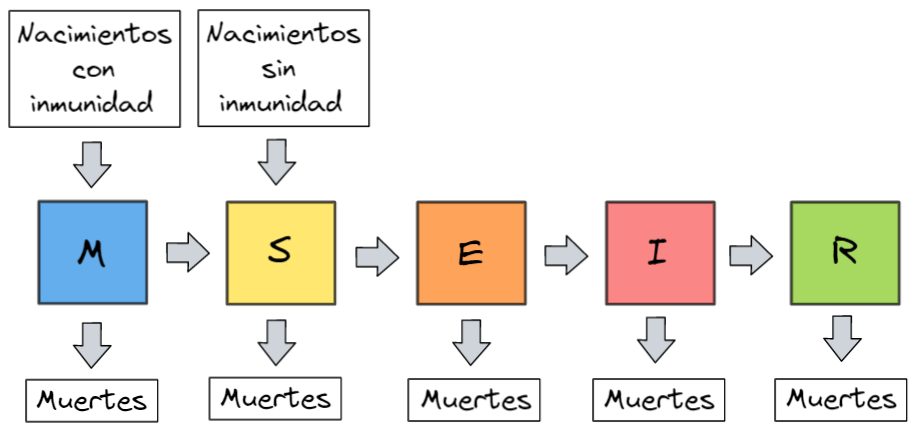
\includegraphics[width=0.7\textwidth]{Imagenes/MSEIR_compatimientos.PNG}
  \caption{Diagrama de compartimientos para el modelo MSEIR}
  \label{fig:diagrama MSEIR}
\end{figure}

Generalmente cuando hablamos de modelos epidemiológicos se consideran tres estados o clases en las que podemos dividir a la población en el tiempo: Los que pueden contraer la enfermedad, los que se infectan y los que se recuperan. Si los que se recuperan no adquieren una inmunidad permanente, nos encontraremos ante un modelo SIS, en el que los susceptibles pueden contraer la enfermedad y una vez se recuperan vuelven al estado de susceptibilidad. Por otro lado, si los individuos que se recuperan generan inmunidad a la enfermedad, estaremos ante un modelo SIR. 

Teniendo en cuenta este tipo de consideraciones nos permitimos establecer a los modelos SIS y SIR como foco principal de nuestra investigación sin dejar a un lado la idea de retomar modelos como el MSEIR para investigaciones futuras. Adicionalmente para efectos aplicables consideraremos las variaciones que tienen en cuenta la natalidad y mortalidad bien sea a causa o por efectos ajenos a la enfermedad.

Brauer y Castillo describen en \cite{mateModelsInPopulationAndEpidemiology} los planteamientos y técnicas para analizar este tipo de modelos. Nos apoyaremos también en el trabajo realizado por Diego de Pereda Sebastián en \cite{diego2010} para algunos resultados y observaciones interesantes sobre cada modelo.

\subsection{El modelo SIS}\label{sub:El modelo SIS}

El modelo SIS considera 2 posibles estados, susceptibles (S) e infectados (I). Las variaciones entre los estados vienen dadas por los nuevos contagios y los individuos que se recuperan de la enfermedad. Adicionalmente, cada estado se ve afectado por los parámetros que describen la natalidad/mortalidad y la muerte a cauda de la enfermedad. 

Los diferentes estados del modelo se pueden apreciar en el diagrama (\ref{fig:diagrama SIS}):

\begin{figure}[h]
  \centering
    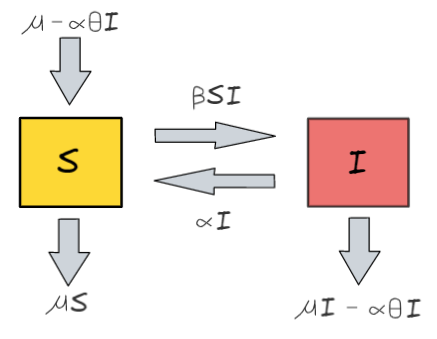
\includegraphics[width=0.4\textwidth]{Imagenes/SIS_compartimientos.PNG}
  \caption{Diagrama de compartimientos para el modelo SIS}
  \label{fig:diagrama SIS}
\end{figure}

Es importante recordar que trabajaremos sobre una población de tamaño constante y normalizado, por lo que $S + I = 1$ y en consecuencia $S' + I' = 0$.

Normalmente cuando se habla de modelos epidemiológicos con muerte por enfermedad se consideran 4 parámetros: 

\begin{itemize}
    \item La \textbf{tasa de infección $\beta$}, que representa la probabilidad que tiene un individuo susceptible de adquirir la enfermedad luego de un contagio con un infectado.
    \item La \textbf{tasa de recuperación $\alpha$}, que podemos entender como la probabilidad de que un infectado se recupere de la enfermedad.
    \item La \textbf{tasa de natalidad/mortalidad $\mu$}, que en el caso de los modelos clásicos se considera igual. La natalidad nos indica la cantidad de individuos que ingresan al espacio y la mortalidad representa los individuos que fallecen por causas ajenas a la enfermedad.
    \item La \textbf{tasa de muerte por enfermedad $\theta$}, que nos indica la probabilidad que tiene un infectado de fallecer a causa de la enfermedad.
\end{itemize}

Podemos describir el modelo a partir de un sistema de ecuaciones diferenciales como sigue:

\begin{equation}\label{eq:Modelo SIS}
\left\{
\begin{array}{l}
S' = \mu(1 - S) + (1 - \theta)\alpha I - \beta S I \\
I' = \beta S I - (1 - \theta)\alpha I - \mu I
\end{array}
\right.
\end{equation}

Para determinar los escenarios bajo los cuales una enfermedad es endémica debemos calcular el valor de $R_0$ para nuestro sistema de ecuaciones diferenciales (\ref{eq:Modelo SIS}). Recuerde que para determinar el valor de $R_0$ se considera una población completamente susceptible, es decir, $S=1$ y $I=0$.

Observe que los nuevos infectados vienen dados por el término $\beta S$, con lo cual definimos $b(t) = \beta S = \beta$. Por otro lado, los flujos que determinan la salida del estado de infección de los individuos viene dado por los términos $-\alpha(1-\theta)I-\mu I$, de modo que si llamamos $I(t)$ a la cantidad de individuos infectados que permanecieron infectados desde el momento 0, tenemos

\begin{equation}\label{eq:Cambio en I}
\frac{dI}{dt} = -\alpha(1-\theta)I-\mu I
\end{equation}

Donde al usar el método de separación de variables obtenemos

\begin{equation}\label{eq:Infectados en el tiempo}
I(t) = I(0)e^{-(\alpha(1-\theta)+\mu)t}
\end{equation}

De ese modo, podemos afirmar que la proporción de individuos que permanecen infectados hasta un tiempo $t$ viene dado por $e^{-(\alpha(1-\theta)+\mu)t}$, con lo cual $F(t)=e^{-(\alpha(1-\theta)+\mu)t}$. Finalmente, al reemplazar en (\ref{eq:R0}) obtenemos:

\begin{align*}
R_0 &= \lim_{T\to\infty}\int_0^T b(t)F(t) dt \\
&= \lim_{T\to\infty}\int_0^T \beta e^{-(\alpha(1-\theta)+\mu)t} dt\\
&= \frac{\beta}{\alpha(1-\theta)+\mu}
\end{align*}

\underline{\textit{Observación:}} De la ecuación (\ref{eq:Infectados en el tiempo}) podemos afirmar que la cantidad de individuos infectados tiende a cero cuando $t$ tiende a infinito.

\subsubsection{Análisis de estabilidad}

Para analizar la estabilidad de nuestro modelo SIS debemos conocer sus puntos de equilibrio. Al anular ambas derivadas nos damos cuenta de que están dados por 

$$P_0=(S_a,I_a)=(1,0), P_1=(S_b,I_b)=\left(\frac{\alpha(1-\theta)+\mu}{\beta},\frac{\beta-\alpha(1-\theta)-\mu}{\beta}\right)$$

Veamos que los puntos de equilibrio satisfacen las condiciones de ser positivos y menores o iguales a 1:

En el caso de $P_0$ la verificación es trivial. Por otro lado, para el caso de $P_1$ observe que 

$$0\leq\alpha(1-\theta)+\mu\leq\beta \longrightarrow \frac{\alpha(1-\theta)+\mu}{\beta}\text{, }\frac{\beta+\alpha(1-\theta)+\mu}{\beta}\geq0$$

Si dividimos la expresión del lado izquierdo por $\beta$ obtenemos

$$0\leq \frac{\alpha(1-\theta)+\mu}{\beta}\leq1$$

De donde podemos afirmar que 

$$1-\frac{\alpha(1-\theta)+\mu}{\beta}\leq1 \longrightarrow \frac{\beta-\alpha(1-\theta)-\mu}{\beta}\leq1$$

De donde podemos concluir que ambos puntos de equilibrio cumplen las condiciones de tener coordenadas positivas y menores que la unidad.

Es momento de determinar los comportamientos que describen ambos puntos, $P_0$ y $P_1$. Consideremos el jacobiano de nuestro modelo:

$$|A-\lambda I|=
\left|\begin{array}{cc}
-\mu-\beta I-\lambda & \lambda(1-\theta)-\beta S \\
\beta I & \beta S-\alpha(1-\theta)-\mu-\lambda
\end{array}\right|$$

Si evaluamos en $P_0$ obtendremos los valores propios

$$\left\{\begin{array}{l}\lambda=-\mu \\
\lambda=\beta-\alpha(1-\theta)-\mu\end{array}\right.$$

Con lo cual, podemos afirmar que si $R_0>1$, $P_0$ se comportará como un punto de silla y por otro lado, si $R_0<1$ estaremos ante un nodo estable. Para el caso de $P_1$ tendremos un comportamiento tipo sumidero dado que $\lambda=0,\lambda=-\mu$ son los valores propios asociados a $P_1$.

\subsubsection{Estudio numérico}

Para representar las soluciones del sistema de ecuaciones diferenciales que describe el modelo SIS usaremos el método de Euler, el cual se implementó en el módulo: "\textit{CompartmentalModelsInEDOS}".

De manera general, dadas unas condiciones iniciales $S(0)=S_0,I(0)=I_0$ aplicamos el método de Euler a partir de la siguiente expresión

$$\left\{\begin{array}{l}
S_{t+1} = S_t + h\cdot(\mu(1 - S_t) + (1 - \theta)\alpha I_t - \beta S_t I_t ) \\
I_{t+1} = I_t + h\cdot(\beta S_t I_t - (1 - \theta)\alpha I_t - \mu I_t)
\end{array}\right.$$

\begin{itemize}
    \item Consideremos por ejemplo una enfermedad en la que la tasa de recuperación $\alpha$ es del $0.2$ y su tasa de infección es de $\beta=0.5$ con una tasa de letalidad de $\theta=0.4$. La tasa de natalidad para nuestra población será de $\mu=\frac{1}{75\cdot365}$, es decir, una esperanza de vida de $75$ años.
    
    \begin{figure}[h]
      \centering
        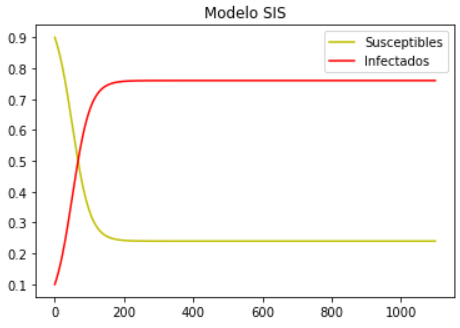
\includegraphics[width=0.4\textwidth]{Imagenes/ex1SIS.PNG}
      \caption{Evolución de la enfermedad en 1100 días con $S_0=0.9,I_0=0.1$ y $h=0.1$.}
      \label{fig:Ejemplo 1 - SIS}
    \end{figure}
\end{itemize}

\subsection{El modelo SIR}\label{sub:El modelo SIR}

Para este modelo se considera el estado de inmunidad frente a la enfermedad R. A diferencia del modelo SIS, en el modelo SIR no hay una interacción del estado I al estado S, ya que se supone que los individuos que se recuperen de la enfermedad no podrán volver a contraerla, por lo que pasaran al estado R. 

En el diagrama (\ref{fig:diagrama SIR}) se pueden apreciar las interacciones para los estados del modelo:

\begin{figure}[h]
  \centering
    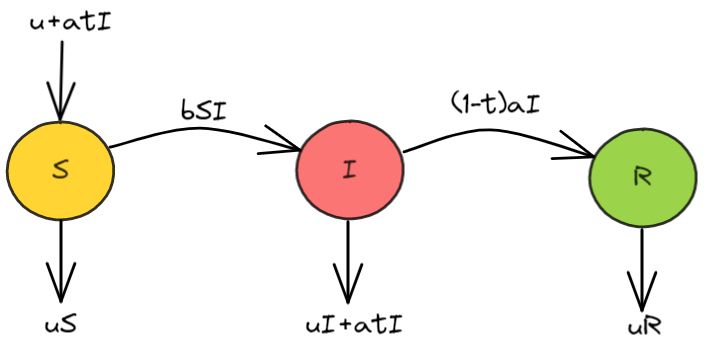
\includegraphics[width=0.7\textwidth]{Imagenes/SIR_compartimientos.PNG}
  \caption{Diagrama de compartimientos para el modelo SIR}
  \label{fig:diagrama SIR}
\end{figure}

De ese modo, el sistema de ecuaciones diferenciales que describe las interacciones entre estados viene dado por la siguiente ecuación:

\begin{equation}\label{eq:Modelo SIR}
\left\{
\begin{array}{l}
S' = \mu(1 - S) + \alpha\theta I - \beta S I \\
I' = \beta S I - \mu I - \theta\alpha I - (1 - \theta)\alpha I = \beta S I - \alpha I - \mu I \\
R' = \alpha I - \alpha\theta I - \mu R
\end{array}
\right.
\end{equation}

En este caso, la ecuación diferencial que describirá la cantidad de individuos infectados desde el momento 0 viene dada por:

\begin{equation}\label{eq:Infectados en el tiempo I - SIR}
    \frac{dI}{dt}=-\mu I - \alpha I \longrightarrow I(t)=I(0)e^{-(\alpha+\mu)t}
\end{equation}

Con lo que definimos $F(t)=e^{-(\alpha+\mu)t}$. Por otra parte, la función $b(t)$ estará definida de la misma manera que en el modelo SIS debido a la manera en la que se describe el modelo. Así, al reemplazar en (\ref{eq:R0}):

\begin{align*}
R_0 &= \int_0^\infty b(t)F(t) dt \\
&= \lim_{T\to\infty} \int_0^T b(t)F(t) dt \\
&= \frac{\beta}{\alpha+\mu}
\end{align*}

\underline{\textit{Observación:}} De acuerdo con la ecuación \ref{eq:Infectados en el tiempo I - SIR}, la población de infectada tendera a cero cuando $t$ tienda a infinito.

\subsubsection{Análisis de estabilidad}

Al igualar a cero las derivadas del sistema de ecuaciones \ref{eq:Modelo SIR} obtenemos los puntos de equilibrio:

$$\begin{array}{cc}
P_0=(S_a,I_a,R_a)=(1,0,0) & P_1=(S_b,I_b,R_b)=\left(\frac{\alpha+\mu}{\beta},\frac{\mu(\beta-\alpha-\mu)}{\beta(\mu+(1-\theta)\alpha)},\frac{(1-\theta)\alpha(\beta-\alpha-\mu)}{\beta(\mu+(1-\theta)\alpha)}\right)
\end{array}$$

Veamos que las coordenadas de ambos puntos cumplen las condiciones de ser positivos y menores o iguales que uno: 

En el caso de $P_0$ se cumple de manera trivial. Por otro lado, como $\alpha,\beta,\theta$ y $\mu$ son valores positivos podemos afirmar que $S_b>0$, para $I_b$ y $R_b$ observe que 

$$\begin{array}{ccc}
\frac{\mu(\beta-\alpha-\mu)}{\beta(\mu+(1-\theta)\alpha)},\frac{(1-\theta)\alpha(\beta-\alpha-\mu)}{\beta(\mu+(1-\theta)\alpha)}>0 & \text{, si} & \beta-\alpha-\mu>0
\end{array}$$

De la ecuación anterior podemos afirmar que 

$$\beta-\alpha-\mu>0\longrightarrow1>\frac{\alpha+\mu}{\beta}$$

Además, como ya sabemos que se trata de un valor positivo podemos deducir que 

\begin{align*}
1&>1-\frac{\alpha+\mu}{\beta} \\
&= \frac{(\beta-\alpha-\mu)(\mu+(1-\theta)\alpha)}{\beta(\mu+(1-\theta)\alpha)}\\
&= \frac{\mu(\beta-\alpha-\mu)}{\beta(\mu+(1-\theta)\alpha)}+\frac{(1-\theta)\alpha(\beta-\alpha-\mu)}{\beta(\mu+(1-\theta)\alpha)}
\end{align*}

Con lo cual,

$$\frac{\mu(\beta-\alpha-\mu)}{\beta(\mu+(1-\theta)\alpha)},\frac{(1-\theta)\alpha(\beta-\alpha-\mu)}{\beta(\mu+(1-\theta)\alpha)}<1$$

Hemos demostrado que ambos puntos de equilibrio cumplen con las condiciones de tener coordenadas positivas y menores a la unidad. Ahora analizaremos la estabilidad de nuestro modelo SIR, consideremos el jacobiano de nuestro sistema de ecuaciones diferenciales:

$$|A-\lambda I|=(-\mu-\lambda)
\left|\begin{array}{cc}
-\beta I-\mu-\lambda & -\beta S+\theta\alpha\\
\beta I & \beta S-\alpha-\mu -\lambda
\end{array}\right|$$

Si evaluamos en el punto $P_1$, podemos identificar un comportamiento de tipo silla si $\beta-\alpha-\mu>0$, en caso contrario nos encontraremos ante un nodo estable.

Si tomamos ahora el punto $P_2$ y observamos los valores propios 

$$\left\{\begin{array}{l}
\lambda=-\mu\\
\lambda=-\frac{1}{2}\frac{\mu\beta-\mu\theta\alpha+\sqrt{(\mu\beta-\mu\theta\alpha)^2-4\mu(\beta-\alpha-\mu)(\alpha+\mu-\theta\alpha)^2}}{\alpha+\mu-\theta\alpha} \\
\lambda=-\frac{1}{2}\frac{\mu\beta-\mu\theta\alpha-\sqrt{(\mu\beta-\mu\theta\alpha)^2-4\mu(\beta-\alpha-\mu)(\alpha+\mu-\theta\alpha)^2}}{\alpha+\mu-\theta\alpha}
\end{array}\right.$$

Y de ese modo obtendremos dos tipos de comportamientos, una espiral estable si los valores propios son imaginarios y un nodo estable en el caso de que los valores propios sean reales.

\subsubsection{Estudio numérico}

De manera general, si usamos el método de Euler dadas las condiciones iniciales $S(0)=S_0,I(0)=I_0$ las expresiones que describen las soluciones discretas son:

$$\left\{\begin{array}{l}
S_{t+1} = S_t + h\cdot(\mu(1 - S_t) + \alpha\theta I_t - \beta S_t I_t) \\
I_{t+1} = I_t + h\cdot(\beta S_t I_t - \alpha I_t - \mu I_t) \\
R_{t+1} = R_t + h\cdot(\alpha I_t - \alpha\theta I_t - \mu R_t)
\end{array}\right.$$

\begin{itemize}
    \item Para este ejemplo supondremos una variación de la enfermedad contemplada en el ejemplo del modelo SIS en la que los individuos que se recuperan de la enfermedad adquieren inmunidad.
    
    \begin{figure}[h]
      \centering
        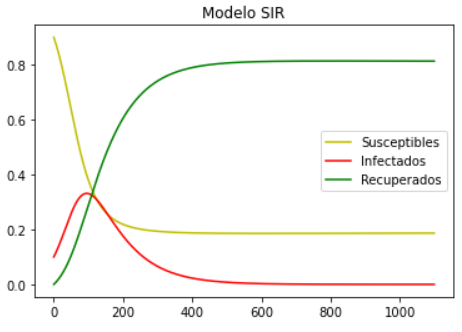
\includegraphics[width=0.4\textwidth]{Imagenes/ex1SIR.PNG}
      \caption{\centering Evolución de la enfermedad en 1100 días con $S_0=0.9,I_0=0.1,R_0=0$ y $h=0.1$.}
      \label{fig:Ejemplo 1 - SIR}
    \end{figure}
\end{itemize}


\chapter{Modelos epidemiológicos en autómatas celulares}\label{ch:Modelos epidemiológicos en AC}

\section{Interacciones e impactos sociales}
A diferencia del trabajo realizado en \cite{populationDensity} en el que cada celda representaba una región, consideraremos a cada división como un único individuo que será dotado de un conjunto de cualidades como estado de salud, edad, vecinos, etc. Estas cualidades vendrán dadas por las necesidades del modelo que estemos desarrollando, por ejemplo en los modelos clásicos no será necesario dotar de edades a las células, pero si tendremos que tener en cuenta sus vecindades y sus estados de salud.

Pensemos por un momento en las características que hay detrás de relación cercana entre individuos o células. Denotaremos la relación entre células con el símbolo $\thicksim$ y una vez dicho esto tenemos que:

\begin{itemize}
    \item Todas las células están en contacto con ellas mismas, por lo que para cada célula $x$ se cumple $x \thicksim x$.
    \item Si una célula estuviera en contacto con alguna otra entonces esa célula estaría en contacto con la primera, es decir, $x\thicksim y$ implica $y\thicksim x$.
    \item Si una célula interactúa con otras dos no implica necesariamente que estas interactúen entre sí, por lo que $x\thicksim y$ y $x\thicksim z$ no implican que $y\thicksim z$.
\end{itemize}

 \textbf{Ejemplo 3.1.1:} Consideremos por ejemplo el conjunto $A=\{a,b,c,d\}$ y a la sub-colección $\mathcal{B} = \{\{a\},\{b\},\{c\},\{d\},\{a,c,d\}, \{b,c\}, \{b,d\}\}$ de $\mathcal{P}(A)$. Claramente se obtienen las siguientes relaciones

$$\begin{array}{cccc}
    a\thicksim a, & b\thicksim b, & c\thicksim c, & d\thicksim d, \\ 
    a\thicksim c, & a\thicksim d, & b\thicksim c, & b\thicksim d,
\end{array}$$

junto con sus relaciones simétricas equivalentes. Esta noción de relación de interacción entre células puede ir un poco más allá. Pensemos por un momento en el impacto que puede tener un comportamiento sobre la célula $b$ en la célula $a$, si bien estas dos celdas no interactúan entre sí, la relación que cada una de ellas tiene con las células $c$ y $d$ puede tener un impacto sobre la otra. Con lo cual definimos la siguiente relación de interacción:

\textbf{Definición 3.1.2:} Definimos el \textit{grado de impacto} entre dos puntos $a$ y $b$ como la menor cantidad de interacciones necesaria para llegar de $a$ a $b$. Para reconocer el grado de impacto entre dos puntos usaremos la notación $a\thicksim_n b$ donde $n\in\mathbb{N}$ denota la menor cantidad de interacciones entre $a$ y $b$.

Si retomamos el ejemplo 3.1.1 podremos identificar los siguientes grados de impacto:

$$\begin{array}{cccc}
    a\thicksim_0 a, & b\thicksim_0 b, & c\thicksim_0 c, & d\thicksim_0 d, \\ 
    a\thicksim_1 c, & a\thicksim_1 d, & b\thicksim_1 c, & b\thicksim_1 d, \\
    a\thicksim_2 b, & c\thicksim_2 d.
\end{array}$$

De la definición anterior se deduce el siguiente resultado:

\textbf{Teorema 3.1.3:} Los grados de impacto de una célula $x$ definen un sistema fundamental de vecindades en la topología discreta.

\begin{proof}
Sea $x\in\mathcal{L}$ y $\mathcal{V}(x)$ una familia de vecindades de $x$. Defina el conjunto $A_0=\{x\}$ como el conjunto de puntos con grado de impacto con $x$ es igual a cero y a continuación defina de manera recursiva a los conjuntos $A_k$ cuyos elementos tienen grado de impacto con $x$ sea igual o menor a $k$. Claramente $A_i\subseteq A_j$ para $0\leq i\leq j$ y de ese modo $A_i\in\mathcal{V}(x)$ para $i=0,1,\cdots,n$.

Defina la colección $\mathcal{A}=\{A_0,A_1,\cdots,A_k,\cdots,A_N\}$ como la familia de conjuntos encajados definidos por el grado de impacto con $x$. Dado que por hipótesis estamos sobre la topología discreta podemos afirmar que para todo $V\in\mathcal{V}(x)$ el conjunto $A_0\subseteq V$ y de ese modo por la definición 2.4.8 concluimos que la colección $\mathcal{A}$ es un sistema fundamental de vecindades de $x$.
\end{proof}

A continuación mostraremos algunas de las propiedades del conjunto $\mathcal{A}$ definido en la demostración anterior:

\textbf{Proposición 3.1.4:} Sea $x\in\mathcal{L}$ una célula y sea $\mathcal{A}$ la familia de conjuntos encajados definidos por el grado de impacto con $x$. Se cumplen las siguientes propiedades:

\begin{enumerate}
    \item El conjunto $\mathcal{A}$ posee elemento mínima igual a $A_0=\{x\}$,
    \item $\mathcal{A}$ es un conjunto ordenado finito con el orden de la contenencia,
    \item $\mathcal{L}$ es un espacio $T_0$, y
    \item $\mathcal{L}$ es un espacio uno-numerable.
\end{enumerate}

\begin{proof}
Cada numeral se deduce directamente de las definiciones 2.4.11, 2.4.13, 2.4.14, 2.4.15, 2.4.16 y el teorema 3.1.3.
\end{proof}

\section{Reglas de evolución}
\subsection{Modelos SIS y SIR simples}
\subsection{Modelos con natalidad y mortalidad}
\subsection{Modelos con muerte por enfermedad}
\section{Comparación con los modelos clásicos}
% \chapter{Conclusiones}

% Al realizar este trabajo se comprendió la manera en que se define la distancia $C^0$,\,la distancia de \textit{Hausdorff},\, la distancia \textit{Gromov-Hausdorff}. Así mismo, cómo se pueden calcular distancias entre objetos en donde estas métricas estén definidas usando las diversas caracterizaciones de distancia, así como propiedades que éstas o los objetos (conjuntos, espacios, funciones) poseen. Posterior a eso, fue posible entender qué motiva y cómo funciona la denominada distancia $GH^0$. Ya con estos conceptos claros, se logró comprender de qué manera difieren o son similares ciertos espacios y/o funciones en términos de qué tan cercanos son con respecto a una forma de definir esa distancia. Luego de eso, fue posible a través del entendimiento del concepto de estabilidad topológica de Walters \cite{WalPOTP}, estudiar la propuesta de $GH$-estabilidad topológica dada por Arbieto \& Morales en \cite{AM}.\\

% Las conclusiones que se pueden enunciar de este trabajo son:
% \begin{itemize}
%     % \item Mediante la introducción de métricas o pseudo métricas es posible estudiar y entender el comportamiento de espacios y sistemas, en el sentido de  comparar con elementos cercanos. A su vez, estudiar fenómenos de convergencia y estabilidad.
%     \item Todo homeomorfismo topológicamente estable es isométricamente estable. Sin embargo el recíproco es falso en general.
%     \item Un homeomorfismo topológicamente $GH$-estable es isometricamente estable. Esto quiere decir que una función $GH$-estable ante pequeñas perturbaciones no solo produce una función con una estructura dinámica, sino que además la dinámica misma de la perturbación es muy cercana. 
%     \item Existe un homeomorfismo el cual es topológicamente estable pero no es topológicamente $GH$-estable. Por ende, la $GH$-estabilidad es una condición distinta de estabilidad.
%     \item Todo homeomorfismo topológicamente $GH$-estable en el circulo es topológicamente estable.
%     \item Todo homeomorfismo  expansivo con la P.O.T.P  de un espacio métrico compacto es topológicamente $GH$-estable (extendiendo el resultado dado por Walters).
%     \item Toda función continua positivamente expansiva con la $P.O.T.P_+$ de un espacio métrico compacto es topológicamente $GH-$estable (Caso no invertible).
%     \item Lo desarrollado en este trabajo sugiere que en espacios compactos la $GH$-estabilidad es una condición más fuerte que la estabilidad topológica. Sin embargo, esto aún no ha sido probado.
% \end{itemize}
% \include{Contenidos/Apéndices}

\addcontentsline{toc}{chapter}{\numberline{}Bibliografía}
  \nocite{*}
  \bibliography{BibliMSc}
  \bibliographystyle{abbrv}
\end{document}